\documentclass[../main/main.tex]{subfiles}

\newdate{date}{25}{10}{2019}


\begin{document}


\chapter{Role of the models in statistical mechanics}
\marginpar{ \textbf{Lecture 6.} \\  \displaydate{date}. \\ Compiled:  \today.}
\section{Role of the models}
Which is the role of models in statistical mechanics? There are two possible approaches:
\begin{enumerate}
  \item The model must describe the real system in a very detailed way. The maximum number of details and parameters to be tuned are included. The \emph{pro} is the closer to the real specific system (faithfull description). The \emph{drawback} is that the model is so complicated that no analytical solution is possible. Moreover, even numerically, these models can be studied for very short times and small sizes.
  An example is the simulation of the folding dynamics that can be performed for few nanoseconds. On the other hand the introduction of many details are often not crucial if one is interested in large scale properties.
  \item Try to introduce the most simple model that satisfies few essential properties of the real system such as its symmetries, dimensionality, range of interactions etc.
  Since most of the microscopic details are integrated, these models cannote describe the full physics of a specific system but they can reproduce its main features. Moreover these models can be studied numerically and, to some extent also analitically (exact solution).
\end{enumerate}
  Let us start by introducing what is, perhaps, the most paradigmatic model in the statistical mechanics of p hase transition, the \emph{Ising model}.

  \section{Ising model (1925)}
  Suggested by Lenz to Ising for his Phd thesis, it is supposed to describe a magnetic system that undergoes a transition between a pramagnetic and a ferromagnetic phase.
  In \( d=1 \) the model was solved exactly by Ising. Unfortunately, he found that for \( T>0 \) the model does not display a phase transition. The wrong conclusion was that this model is not able to describe a phase transition. In fact, it turns out that, for \( d>1 \), the model does display a paramagnetic-ferromagnetic phase transition.  Let us first discuss some general feature of the model for any dimension \( d \).

\subsection{D-dimensional Ising model}
For hypercubic lattice with  given \( N(\Omega ) \) sites \( \{ i \}_{i=1,\dots,N(\Omega )}   \) and linear size \( L(\Omega ) \) , we have \( N (\Omega ) = L^D \). The microscopic degrees of freedom are the spins \( S_i \) defined at each i-esim lattice site. Each spin can assume the values  \( S_i = \pm 1 \), that means that at each site the possible values are the spin up or down. The minimal model that can try to capture the interaction between the spin is the following.

For a lattice with \( N(\Omega ) \) spins, there are \( 2^{N(\Omega )} \)  possible configurations.
\begin{remark}
Since we do not consider the spin as a vector, this is a model for a strongly anysotropic ferromagnet (along a given direction).
\end{remark}
Suppose to have also an external magnetic field \( H_i \) (it values depends on the site \emph{i}). One can consider interactions between spins whose strength are described by functions \( J_{ij},k_{ijk}, \dots \). For instance, there is a coupling that derives from electrons coupling \( J_{ij} = f ( \abs{\va{r_i}- \va{r_j}  } ) \)

The physical origin is the overlap between the electronic orbitals of the neighbouring atoms forming the Bravais lattice.
Remember that a term as \( \sum_{i}^{} S_i  \) is not correlated, while we need an interaction.

A general Hamiltonian of the model can be written as
\begin{equation}
  \mathcal{H}_ \Omega ( \{ S_i \}  ) = \sum_{ij}^{} J_{ij} S_i S_j - \sum_{i}^{} H_i S_i - \sum_{ijk}^{} S_i S_j S_k + \dots
\end{equation}
Standard Ising model one keeps only the two-body interactions:
\begin{equation}
  \mathcal{H}_ \Omega ( \{ S_i \}  ) = -\frac{1}{2}\sum_{i\neq j}^{N} J_{ij} S_i S_j - \sum_{i=1}^{N} H_i S_i
\end{equation}
where the first second is a one body interaction, while in the first term we consider the two body interaction that is a quadratic term. We have put the minus because we want to minimize the energy, but it dipends on the sign of  \emph{J}.

For this model the sum over all configurations on trace is given by
\begin{equation}
  \Tr \equiv \sum_{S_1 = \pm }^{}  \sum_{S_2 = \pm }^{}  \dots \sum_{S_N = \pm }^{} \equiv \sum_{\{ S \}  }^{}
\end{equation}
 Our problem is to find the partition function with \emph{N} sites, which depends on \emph{T} and in principle depends in the configuration given (it is fixed both for \emph{H} and \emph{J}!).
Hence the canonical partition function is given by
\begin{equation}
  Z_{\Omega } (T, \{ H_i \}, \{ J_{ij} \}    ) = \Tr e^{-\beta \mathcal{H}_ \Omega ( \{ S \}  )}
\end{equation}
and the corresponding free-energy
\begin{equation}
  F_ \Omega  (T, \{ H_i \}, \{ J_{ij} \} ) = - k_B T \ln{Z_ \Omega }
\end{equation}
The bulk limiting free energy is
\begin{equation}
  f_b (T, \{ H_i \}, \{ J_{ij} \} ) = \lim_{N \rightarrow \infty } \ln {\frac{1}{N} F_ \Omega  }
\end{equation}
How do we know that the above limit does exist? It must be proven. The surface is not important in the bulk limit.
 Note that we are assuming that the interaction between the spin is a short range force, it is not as the size of the system.

For this model it is possible to show that the limit exists if
\begin{equation}
  \sum_{j \neq i}^{} \abs{J_{ij}} < \infty
\end{equation}
\begin{remark}
In general what determines the existence of the limit of these spin models are the dimension \emph{D} and the range of the spins interactions.
\end{remark}
For example it is possible to show that, if
\begin{equation}
  J_{ij} = A \abs{\va{r_i}-\va{r_j}  }^{-\sigma}
\end{equation}
(so it is a long range interaction)
the limit exists when
\begin{equation}
  \sigma > D
\end{equation}
\begin{remark}
If the interaction is \emph{dipolar} since it decades as \( 1/r^3 \), for the case \( d=3 \) the limit does not exists. However it is still possible to prove the existence of the limit for this case if one assumes that not all dipoles are fully aligned.
\end{remark}
Assuming that the thermodynamic limit exists we now look at some additional rigorous results on the limiting free energy and its derivatives.

\subsection{Mathematical properties of the Ising model with neirest neighbours interactions}
For simplicity let us consider the case in which the external magnetic field is homogeneous i.e. \( H_i \equiv H \) and the spin-spin interaction is only between spins that are nearest-neighbours on the lattice:
\begin{equation}
J_{ij} =
  \begin{cases}
  J & \text{if } i \text{ and } j \text{ are neirest neighbours} \\
  0 & \text{otherwise}
  \end{cases}
\end{equation}

The model is nowe very simple:
\begin{equation}
  - \mathcal{H}_ \Omega ( \{ S \}  ) = J \sum_{\expval{ij} }^{N (\Omega )} S_i S_j + H \sum_{i}^{N(\Omega )} S_i
\end{equation}
where the notation \( \expval{ij}  \) means a double sum over \emph{i} and \emph{j}, with the constraint that \emph{i} and \emph{j} are nearest-neighboyrs.
Since \emph{H} is uniform, the average magnetization per spin is
\begin{equation}
  \expval{m} = \frac{1}{N (\Omega )} \sum_{i=1}^{N (\Omega )} \expval{S_i}
\end{equation}
where \( \expval{\dots}  \)  means average over the chosen ensemble.
Since
\begin{equation}
  \sum_{i=1}^{N} \expval{S_i} = \frac{1}{Z} \Tr \qty[(\sum_{i}^{} S_i ) e^{-\beta \mathcal{H}_ \Omega (\{ S_i \}  )} ]  = \frac{1}{Z} \Tr \qty[\sum_{i}^{} S_i \exp (\beta  J \sum_{\expval{ij} }^{} S_i S_j + \beta H \sum_{i}^{} S_i  )  ]
\end{equation}
it is easy to show that:
\begin{equation}
  \expval{m} = - \frac{1}{N} \pdv{F_ \Omega }{H}
\end{equation}
where
\begin{equation}
  F_ \Omega (T,J,H) = - k_B T \ln{Z_N (T,J,H)}
\end{equation}

Let us now consider the properties of the limiting free-energy
\begin{equation}
  f_b = \lim_{N \rightarrow \infty } \frac{1}{N} (-k_B T \ln{Z_N} )
\end{equation}
It is possible to prove the following properties
\begin{enumerate}
\item \( f_b < 0 \).
\item \( f_B (T,J,H) \) is a continuous function of \emph{T,J} and \emph{H}.
\item The right and left derivatives of \( f_b (T,J,H) \) exist and are equal almost everywhere.
\item The molar entropy \( s = - \pdv{f_b}{T} \ge 0\)    almost everywhere.
\item \( \pdv{f_b}{T}  \) is a monotone non increasing function of \emph{T}. That is \( \pdv[2]{f_b}{T} \le  0 \). In particular this implies that:
\begin{equation}
  c_H = T \qty(\pdv{S}{T} )_M = - T \qty(\pdv[2]{f_b}{T} \ge 0)
\end{equation}
\item \( \pdv{f_b}{H}  \) is a monotonic non increasing function of \emph{H}. That is
\begin{equation}
  \pdv[2]{f_b}{H} \le 0
\end{equation}
This implies that
\begin{equation}
  \chi _T = \qty(\pdv{M}{H} )_T = - \qty(\pdv[2]{f_b}{H})_T \ge 0
\end{equation}
\end{enumerate}
\begin{remark}
The above properties have been postulated in thermodynamics but here it has been rigorously proved for the Ising model using statistical mechanics.
\end{remark}
\begin{proof} [Proof of property (4)]
  Almost everywhere we have to prove that:
  \begin{equation}
    s \equiv - \pdv{f_b}{T} \ge 0
  \end{equation}
  Let us consider a finite system
  \begin{equation}
  \begin{split}
  - \pdv{F_ \Omega }{T}   &= k_B \ln{(\Tr e^{- \beta \mathcal{H}_ \Omega }  )} + k_B T \frac{1}{k_B T^2} \frac{\Tr(\mathcal{H}_ \Omega  e^{-\beta \mathbb{H}} ) }{\Tr(e^{- \beta \mathcal{H}} ) } \\
  &= k_B \qty[\ln{Z} + \frac{\Tr(\beta \mathcal{H}_ \Omega e^{-\beta \mathcal{H}_ O
  } ) }{Z_ \Omega } ] =  - k_B T \Tr(\rho _ \Omega  \ln{\rho _ \Omega } )
  \end{split}
  \end{equation}
  where  we used the definition of the probability distribution
  \begin{equation}
    \rho _ \Omega  = \frac{e^{-\beta \mathcal{H}_ \Omega } }{Z A } (????)
  \end{equation}
  Since \( \rho _ \Omega \le 1 \) it implies \( \ln{\rho _ \Omega } \le 0  \) and so \( - \Tr(\rho _ \Omega ) \ln{\rho _ \Omega }   \) is positive. Let us divide by \( N (\Omega ) \) and take the thermodynamic limit:
  \begin{equation}
  \lim_{N \rightarrow \infty } - \frac{1}{N} \pdv{F_ \Omega }{T}   = - k_B T  \lim_{N \rightarrow \infty }  \frac{1}{N}  \underbrace{\Tr(\rho _ \Omega  \ln{\rho _ \Omega })}_{S _ \Omega }  = T s \ge 0  \quad \Rightarrow \quad s \ge 0
  \end{equation}
\end{proof}
All the other properties listed before (except \( (a) \)) are consiquences of the \emph{convexity} property of \( f_b \)
\begin{theorem}[]
\( f_b  (T,J,H)\) is an upper convex (i.e. concave) function of \emph{H}.
\end{theorem}
\begin{proof}
The proof is based on the H$\ddot{o}$lder inequality for two seuqnces  \( \{ g_k \}, \{ h_k \}     \).
\begin{definition}[H$\ddot{o}$lder inequality]
  Given  \( \{ g_k \}, \{ h_k \}     \) with \( g_k,h_k \ge 0, \forall k \) and two non negative real numbers \( \alpha _1, \alpha _2 \) such that \( \alpha _1 + \alpha _2 =1 \), the following inequality holds
  \begin{equation}
    \sum_{k}^{} (g_k)^{\alpha _1} (h_k)^{\alpha _2} \le \qty(\sum_{k}^{} g_k )^{\alpha _1} \qty(\sum_{k}^{} h_k )^{\alpha _2}
  \end{equation}
\end{definition}
Consider now the partiction function
\begin{equation}
  Z_ \Omega  (H) = \Tr[\exp (\beta H \sum_{i}^{} S_i ) \underbrace{\exp (\beta J \sum_{\expval{ij} }^{} S_i S_j ) }_{G (S)}  ] = \Tr [\exp (\beta H \sum_{i}^{} S_i ) G (s)]
\end{equation}
it implies that
\begin{equation}
  Z_ \Omega  (H_1 \alpha _1 + H_2 \alpha _2) = \Tr(\exp {\beta \alpha _1 H_1 \sum_{i}^{} S_i + \beta \alpha _2 H_2 \sum_{i}^{} S_i} G(S))
\end{equation}
On the other hand, since \( \alpha _1 + \alpha _2 =1 \):
\begin{equation}
  G (S) = G (S)^{\alpha _1} G(S)^{\alpha _2}
\end{equation}

\begin{equation}
    Z_ \Omega  (H_1 \alpha _1 + H_2 \alpha _2)   = \Tr[ (e^{\beta H_1 \sum_{i}^{} S_i } G (S))^{\alpha _1} (e^{\beta H_2 \sum_{i}^{} S_i } G (S))^{\alpha _2}]
\end{equation}
If we now apply the H$\ddot{o}$lder inequality we get
\begin{equation}
\begin{split}
    Z_ \Omega  (H_1 \alpha _1 + H_2 \alpha _2) & \le \qty(\Tr (e^{\beta H_1 \sum_{i}^{} S_i } G(S))^{\alpha _1}  ) \qty(\Tr (e^{\beta H_2 \sum_{i}^{} S_i } G (S))^{\alpha _2}  ) \\
    & = Z_ \Omega (H_1)^{\alpha _1} Z_ \Omega (H_2)^{\alpha _2}
\end{split}
\end{equation}
If we now take the logs and multiply by \( -k_B T \) both sides we have
\begin{equation}
  \lim_{N \rightarrow \infty } - \frac{1}{N} k_B T \ln{Z_ \Omega (H_1 \alpha _1 + H_2 \alpha _2)}  \ge
   - \lim_{N \rightarrow \infty } \frac{\alpha _1}{N} k_B T \ln{Z_ \Omega  (H_1 )} -
    \lim_{N \rightarrow \infty } \frac{\alpha _2}{N} k_B T \ln{Z_ \Omega  (H_2 )}  \\
\end{equation}
It implies
\begin{equation}
  f_b (H_1 \alpha _1 + H_2 \alpha _2) \ge \alpha _1 f_b (H_1 ) +  \alpha _2 f_b (H_2)
\end{equation}
That is a concave function of \emph{H}.
\end{proof}
\subsection{Ising model and \( \mathcal{Z}^2 \) symmetry. }
The symmetry of the system in sense of the Hamiltonian is: you can invert the value of the \emph{S} and the Hamiltonian does not change. It is valid when \( H=0 \) (? or T is at the critical point booh). Otherwise is not true. Let us see this Z symmetry.
Another interesting relation is the following:
\begin{lemma}[]
\( \forall  \) function \( \Phi  \) of the configuration \( \{ S_i \}   \) the following relation holds
\begin{equation}
  \sum_{ \{S_i = \pm 1\}}^{}  \Phi  (\{S_i\} ) =   \sum_{ \{S_i = \pm 1\}}^{}  \Phi  (\{-S_i\} )
    \label{eq:6_1}
\end{equation}
this is true for all function of the spin.
\end{lemma}
We now consider the Hamiltonian of the Ising model:
\begin{equation}
  - \mathcal{H}_ \Omega  = J \sum_{\expval{ij} }^{} S_i S_j + H \sum_{}^{} S_i
\end{equation}
Clearly
\begin{equation}
  \mathcal{H}(H,J, \{S_i\}) =   \mathcal{H}_ \Omega (-H,J, \{-S_i\})
  \label{eq:6_1_1}
\end{equation}
This is a spontaneous broken symmetry. Hence
\begin{equation}
  \begin{split}
Z_ \Omega  (-H,J,T) &= \sum_{ \{S_i = \pm 1 \}}^{} \exp [-\beta \mathcal{H}_ \Omega  (-H,J, \{S_i\})]  \underset{\eqref{eq:6_1}}{=}   \sum_{ \{S_i = \pm 1 \}}^{} \exp [-\beta \mathcal{H}_ \Omega  (-H,J,\{-S_i\})] \\
&\underset{\eqref{eq:6_1_1}}{=} \sum_{ \{S_i= \pm 1\}}^{} \exp [-\beta \mathcal{H}_ \Omega  (H,J, \{S_i\}) ] = Z_ \Omega (H,J,T)
\end{split}
\end{equation}
Taking \( -k_B T \log  \)  and the \( \lim_{N \rightarrow \infty } \frac{1}{N} \)  we got
\begin{equation}
  F_ \Omega  (T,J,H) = F_ \Omega  (T,J,-H)
  \label{eq:6_2}
\end{equation}
If we now take the thermodynamic limit we have
\begin{equation}
\Rightarrow f_b (T,J,H) = f_b (T,J,-H)
\end{equation}
It means that the free energy density is an even function of \emph{H}!
\begin{remark}
From the finite-size relation \eqref{eq:6_2} one can show that a finite-size Isin model does not displat a transition to a ferromagnetic phase (for all dimension \emph{D}). Indeed
\begin{equation}
    N (\Omega ) M(H) = - \pdv{F (H)}{H} \underset{\eqref{eq:6_2}}{=}  - \pdv{F(-H)}{(H)} = \pdv{F_N(-H)}{(-H)}  = - N (\Omega ) M (-H)
\end{equation}
Therefore:
\begin{equation}
  M (H) = - M (-H) \quad \forall H
\end{equation}
If \( H=0 \), we have \( M (0) = -M (0) \), that is valid if and only if \( M(0)= 0 \)!

The magnetization of a finite system is, at \( H=0 \), always zero. This is simply consequence of the symmetry argument shown above. It is only in the thermodynamic limit where the symmetry is spontaneously broken.
\end{remark}

\subsection{Lattice gas model}
Even if you haven't seen any transition, it is an interesting model because we can use this model to solve other problems that seems different. In fact, the importance of the Ising model relies also on the fact that it can be mapped into other discrete systems. One of these is the \emph{lattice gas model}, where a gas is put in a lattice.
 What is a lattice gas model?
 Let us consider a \emph{d}-dimensional lattice with coordination number \emph{z} and lattice spacing \emph{a}, divided into cell as in Figure \ref{fig:6_1} . Let us suppose that each cell is either empty or occupied by a single particle (this is more true if \( a \sim \SI{}{\angstrom}  \)).
 \begin{figure}[h!]
 \centering
 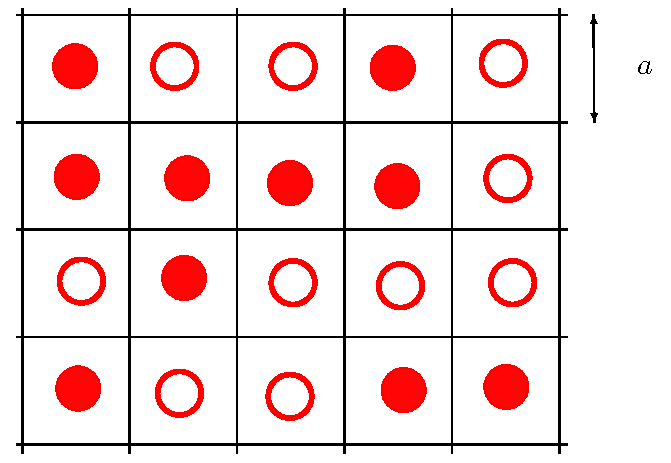
\includegraphics[width=0.6\textwidth]{../lessons/6_image/1.pdf}
 \caption{\label{fig:6_1} Description.}
 \end{figure}
 The \( n_i \) is the occupation of the i-esim cell and it is
\begin{equation}
n_i =
  \begin{cases}
   0 & \text{if empty} \\
   1 & \text{if occupied}
  \end{cases}
\end{equation}
\begin{equation}
  N _ \Omega = \sum_{i=1}^{N_c} n_i
\end{equation}
where \( N_c \) is the number of the lattice cells. In particular, \( N_c > N \).
The hamiltonian of the model is
\begin{equation}
  \mathcal{H}_ \Omega  = \sum_{i=1}^{N_c} U_1 (i) n_i + \frac{1}{2} \sum_{ij}^{} U_2 (i,j) n_i n_j + O (n_i n_j n_k)
\end{equation}
where \( U_1 \) is an external field for instance, while \( U_2 \) is a many body interaction.
Since we want to work in the gran-canonical ensemble
\begin{equation}
  \mathcal{H}_ \Omega  - \mu N = \sum_{i=1}^{N_c} ( \cancel{ U_1 (i)} - \mu) n_i + \frac{1}{2} \sum_{ij}^{} U_2 (i,j) n_i n_j +   \dots
\end{equation}
we put \( U_1=0 \) for convenience. A formal relation with the Ising model can be obtained by choosing
\begin{equation}
  n_i = \frac{1}{2} (1+S_i) \quad \text{with } S_i = \pm 1
\end{equation}
The one body term:
\begin{equation}
  \sum_{i}^{} (U_1 (i) - \mu )  \frac{1}{2} (1+S_i) = \frac{1}{2} \sum_{i}^{} (U_1 (i) - \mu ) + \frac{1}{2} \sum_{i}^{} S_i (U_1 (i) - \mu )
\end{equation}
while the two bies term:
\begin{equation}
  \frac{1}{2} \sum_{ij}^{} U_2 (i,j) \qty[\frac{1}{4} (1+S_i)(1+S_j)] = \frac{1}{8} 2 \sum_{ij}^{N_c} U_2 (i,j) S_i + \frac{1}{8}  \sum_{ij}^{N_c} U_2 (i,j) S_i S_j + \frac{1}{8} \sum_{ij}^{N_c} U_2 (i,j)
\end{equation}
Let us consider only short-range interactions, i.e.
\begin{equation}
U_2 (i,j) =
  \begin{cases}
   U_2 & i,j \text{ neirest neighbours}\\
   0 & \text{otherwise}
  \end{cases}
\end{equation}
It implies
\begin{equation}
  \frac{1}{8} U_2 Z N_c + \frac{1}{4} z U_2 \sum_{i}^{N_c} S_i + \frac{U_2}{4} \sum_{\expval{ij} }^{} S_i S_j
\end{equation}
Remember that we put \( U_1 = 0 \) for simplicity:
\begin{equation}
    \mathcal{H}_ \Omega  - \mu N  =  E_0 - H \sum_{i=1}^{N} S_i - J \sum_{\expval{ij} }^{} S_i S_j
\end{equation}
where
\begin{subequations}
\begin{align}
     E_0 & = - \frac{1}{2} \mu N_c + \frac{z}{8} U_2 N_c \\
       H &= - \frac{1}{2} \mu + \frac{z}{4} U_2 \\
         -J & = \frac{U_2}{4}
\end{align}
\end{subequations}
where remember that \emph{z} is the coordination number of neighbours. It implies
\begin{equation}
  \mathcal{Z}_{LG} = \Tr_{\{n\}}(e^{-\beta (\mathcal{H}_ \Omega -\mu N)} ) = e^{-\beta E_0} Z_{\text{Ising}} (H,J,N_c)
\end{equation}
We have seen that the Ising model is something more general than the magnetization transition.
In the next section we show how to pass from the partition \( \mathcal{Z} \) of a fluid in the continuum to the  \( \mathcal{Z}_{LG} \) of the lattice gas model.
\section{Fluid system in a region \( \Omega  \) }
We can consider the system with periodic boundary condition or within a box or confined by an external one-body potential. The hamiltonian for \emph{N} particles in \emph{D}-dimension is
\begin{equation}
  \mathcal{H}_ \Omega = \sum_{i=1}^{N} \qty[\frac{p_i^2}{2m} + U_1 (\va{r_i})] + \frac{1}{2} \sum_{i \neq j}^{} U_2 (\va{r_i}, \va{r_j}) + \frac{1}{3!} \sum_{i \neq j \neq k }^{}  U_3 (\va{r_i}, \va{r_j}, \va{r_k})
\end{equation}
In the gran-canonical ensemble
\begin{equation}
  \mathcal{Z}_ \Omega = \Tr(e^{-\beta (\mathcal{H}_ \Omega  - \mu N)} ) = \sum_{N=0}^{\infty } \frac{1}{N!} \int_{}^{} \prod_{i=1}^{N} \frac{\dd[D]{\va{p_i}} \dd[D]{\va{r_i}} }{h^{dN}} \qty(e^{-\beta (\mathcal{H}_ \Omega  - \mu N)} )
\end{equation}
and the gran-canonical potential
\begin{equation}
  \omega _ \Omega (T, \mu , U_1, U_2, \dots) = -k_B T \ln{\mathcal{Z}_ \Omega }
\end{equation}
\begin{remark}
\( \omega _ \Omega (\dots) \) even if it contains an infinite sum is not singular if \( \Omega  \) is finite!
\end{remark}
Indeed if \( U_2 \) is an hard-core repulsion, each particle has a finite volume and, within a finite \( \Omega  \), only \( N_{max} \) particles can fit in
\begin{equation}
  \Rightarrow \sum_{N=0}^{\infty } \sim \sum_{N=0}^{N_{max}}
\end{equation}

In the thermodynamic limit
\begin{equation}
  \omega _ b (T, \mu , U_1, U_2, \dots) = \lim_{V (\Omega ) \rightarrow \infty } \frac{o
  _ \Omega }{V (\Omega )}
\end{equation}
with the contraint
\begin{equation}
  \rho = \lim_{V \rightarrow \infty } \frac{\expval{N} }{V (\Omega ) } = const
\end{equation}
remember also that
\begin{equation}
\dd[]{\omega _b (T, \mu )} = - \sigma \dd[]{T} - p \dd[]{\mu } = - P
\end{equation}
Now:
\begin{equation}
  \mathcal{Z}_N = \sum_{N=0}^{\infty } \frac{1}{N!} \qty[\prod_{i=1}^{N}  \qty{ \int_{-\infty }^{+ \infty } \dd[D]{\va{p}} \frac{1}{h^{DN}} e^{-\beta \va{p_i}^2/2m}  } Q_N (T) ]
\end{equation}
On the other hand since \( \int_{}^{} \dd[]{x} e^{- \alpha x^2} = \sqrt{2 \pi / \alpha }    \)
\begin{equation}
  \int_{-\infty }^{+ \infty } \dd[D]{\va{p}} \frac{1}{h^{DN}} e^{-\beta \va{p_i}^2/2m} = \frac{1}{\Lambda (T)^d}
\end{equation}
where
\begin{equation}
  \Lambda ( T) = \frac{1}{\sqrt{2 \pi m k_B} T}
\end{equation}
Therefore:
\begin{equation}
  \mathcal{Z}_ \Omega = \sum_{N=0}^{\infty } \frac{1}{N!} \qty(\frac{e^{\beta \mu } }{\Lambda (T)^d})^N Q_N
\end{equation}
where
\begin{equation}
  Q_N (T) = \int_{}^{} \prod_{i=1}^{N}  \dd[]{\va{r_i}}  e^{-\beta (U(\va{r}))}
\end{equation}
\subsection{From the continuous to the lattice gas model}
Let us divied \( \Omega  \) in discrete cells of size \emph{a}. If \emph{a} is approximate a repulsive range between particles we have that the probability that there is more than a particles sits in a cell is \( \ll 1 \). The potentials of the continuoum model depend on  \( \{ \va{r_i} \}   \).
Consider \( n_ \alpha = n_ \alpha (\va{r_i}) \) the occupation numbers. We have
\begin{equation}
  \sum_{\alpha }^{} n_ \alpha = N = \int_{}^{} \dd[D]{\va{r}} \sum_{i=1}^{N} \delta (\va{r_i}-\va{r})= \int_{}^{} \dd[]{\va{r}} \rho (\va{r})
\end{equation}
where
\begin{equation}
  \rho (\va{r}) = \sum_{i=1}^{N}  \delta (\va{r_i}-\va{r})
\end{equation}
\begin{equation}
  \sum_{i}^{} U_1 (\va{r_i}) = \sum_{i}^{} \int_{\Omega }^{} \dd[D]{\va{r}} U_1 (\va{r})   \delta (\va{r_i}-\va{r}) = \int_{\Omega }^{} \dd[]{\va{r}}      U_1 (\va{r}) \rho (\va{r})
\end{equation}
We have \( U (\{ \va{r_i} \}  ) \rightarrow U (\{ n_ \alpha  \}  ) \) :
\begin{equation}
  Q_N \propto \int_{}^{} \prod_{i=1}^{N}  \dd[D]{\va{r_i}}   \rightarrow \sum_{\{ n_ \alpha  \} }^{}
\end{equation}
Indeed, for each configuration specified bt the set \( \{ n_ \alpha  \}  \) there are \( N! \) possible configurations of \( \{ \va{r_i} \}  \). This is because the particles can exchange position between occupied cells.
Hence \(   Q_N \propto \int_{}^{} \prod_{i=1}^{N}  \dd[D]{\va{r_i}} \simeq N! (a^D)^{N_c} \sum_{\{ n_ \alpha = 0, 1 \}}^{'} \dots  \).
\begin{remark}
The symbol \( \sum_{}^{'}   \) means that the sum has the contraint that the toal number of particles is fixed to \emph{N}.
\end{remark}
\begin{equation}
  Q_N \propto N! (a^D)^N \sum_{\{ n_ \alpha  \} }^{'} e^{-\beta U ( \{ n_ \alpha  \} )}
\end{equation}
\begin{equation}
  \mathcal{Z}_N = \sum_{N=0}^{\infty } \frac{1}{N!} \qty(\frac{e^{\beta \mu } }{\Lambda ^D (T)}) ^N Q_N = \sum_{N=0}^{\infty } \qty[\qty(e^{\beta \mu} \frac{a}{\Lambda (T)}  )^D ]  ^N \sum_{\{ n_ \alpha  \} }^{'} e^{-\beta U ( \{ n_ \alpha  \} )}
\end{equation}
where \( \sum_{}^{'} = \sum_{\{ n_ \alpha  \} }^{}     \)  with the contraint \( \sum_{\alpha }^{} n_ \alpha = N   \).
\begin{remark}
In general it is difficult to perform sum with contraints. Fortunately, we are considering the gran-canonical ensemble.
Indeed we can write
\begin{equation}
  \sum_{N=0}^{\infty} \sum_{\{ n_ \alpha  \}}^{'} f(n_ \alpha ) =   \underset{\sum_{\alpha }^{} n_ \alpha =0 }{\sum_{\{ n_ \alpha  \} }^{'}} f (n_ \alpha )  +
  \underset{\sum_{\alpha }^{} n_ \alpha =1 }{\sum_{\{ n_ \alpha  \} }^{'}} f (n_ \alpha )
  \dots +
    \underset{\sum_{\alpha }^{} n_ \alpha = \infty }{\sum_{\{ n_ \alpha  \} }^{'}} f (n_ \alpha ) =  \sum_{\{ n_ \alpha  \}} f(n_ \alpha )
\end{equation}
with no restriction.
\end{remark}
\begin{remark}
In the final sum all the \( 2^N \) possible microscopic states are inclued (considering \( U_1 =0 \) ):
\begin{equation}
  \mathcal{Z}_ \Omega ^{GC} \propto  \sum_{\{ n_ \alpha  \}} \exp [-\beta \qty(-\mu - \frac{D}{\beta } \log{\frac{a}{\Lambda }} ) \sum_{\alpha =0}^{N_c} n_ \alpha  + \beta U_2 \sum_{\expval{\alpha \beta } }^{} n_ \alpha n_ \beta + \dots     ]
\end{equation}
\begin{equation}
  \mathcal{Z}_ \Omega = \Tr e^{-\beta ( \mathcal{H}_ \Omega - \widetilde{\mu} N )} = Z_{LG} ( \widetilde{\mu } )
\end{equation}
where
\begin{equation}
  \widetilde{\mu } = \mu _{LG} = \mu _{phys} + D k_B T \log{\frac{a}{\Lambda }}
\end{equation}
\end{remark}
%%%%%%%%%%%%%
\clearpage


\section{Ising Model}



\section{Ising d=1}
The Bravais lattice is just a one dimensional lattice (Figure 2) and the partition function is ( we solve it in the case \( H=0 \) ):
\begin{equation}
  Z_N (T) = \sum_{S_1 = \pm 1}^{} \sum_{S_2 = \pm 1}^{} \dots  \sum_{S_N = \pm 1}^{} \exp [
  \overbrace{ \beta J}^{K}  \sum_{i=1}^{N-1} S_i S_{i+1}  ]
\end{equation}
the two body interaction is the sum in all the neighbours that in that case are \emph{i-1} and \emph{i+1}, but you have only to consider the one after, because the one behind is yet taken by the behind site. Solve now this partition function.
Consider \emph{free boundary} condition, therefore the \emph{N} does not have a \emph{N+1}, almost for the moment. We have
\begin{equation}
   K \equiv \beta J,  \quad h \equiv \beta H
\end{equation}
What if we just add another spin at the end \( S_{N+1} \) ? Which is the partition function with that spin ?
\begin{equation}
  Z_{N+1} (T) =   \sum_{S_{N+1} = \pm 1}^{} \sum_{S_1 = \pm 1}^{} \sum_{S_2 = \pm 1}^{} \dots  \sum_{S_N = \pm 1}^{} e^{K (S_1 S_2 + S_2 S_3 + \dots + S_{N-1}S_N)} e^{K S_N S_{N+1}}
\end{equation}
This sum is just involve this term:
\begin{equation}
   \sum_{S_{N+1} = \pm 1}^{} e^{K S_N S_{N+1}}  = e^{K S_N} + e^{-K S_N} = 2 \cosh (K S_N) = 2 \cosh(K)
\end{equation}
\begin{equation}
  Z_{N+1} (T) = (2 \cosh (K) ) Z_N (T)
\end{equation}
\begin{equation}
  Z_{N} (T) = (2 \cosh (K)) Z_{N-1} (T)
\end{equation}
In general, we get:
\begin{equation}
  \Rightarrow Z_N (T) = Z_1 (2 \cos(K) )^{N-1} \quad \text{with} \quad Z_1 = \sum_{S_1=\pm1}^{} 1 = 2
\end{equation}
therefore
\begin{empheq}[box=\myyellowbox]{equation}
  Z_N (T) = 2 ( 2 \cosh (K) )^{N-1}
\end{empheq}
\begin{equation}
  F_N (T) = - k_B T \ln{Z_N (T)} = - k_B T \ln{2} - k_B T (N-1) \ln{2 \cosh (K)}
\end{equation}
\begin{equation}
  f_b \equiv \lim_{N \rightarrow \infty } \frac{1}{N} F_N = -k_B T \ln{ 2 \cosh (\frac{J}{k_B T})}
\end{equation}
The function goes as Figure 3.

Now introduce another way to introduce the same story: compute the magnetization analitic again. Magnetization is the average over spin. Assume \( S_i = \pm 1 \) :
\begin{equation}
  \exp [ k S_i S_{i+1}] = \cosh ( K) + S_i S_{i+1} \sinh (K) = \cosh (K) [1+ S_i S_{i+1} \tanh (K)]
\end{equation}
It means that
\begin{equation}
  Z_N (T) = \sum_{S_1 = \pm 1}^{} \sum_{S_2 = \pm 1}^{} \dots  \sum_{S_N = \pm 1}^{} \exp [
  K  \sum_{i=1}^{N-1} S_i S_{i+1}  ]  \Rightarrow  \sum_{S_1 = \pm 1}^{} \dots  \sum_{S_N = \pm 1}^{} \prod_{i=1}^{N-1} [ \cosh (K) (1+ S_i S_{i+1} \tanh (K))]
\end{equation}
\begin{equation}
  = (\cosh K)^{N-1} \sum_{\{S\}}^{}  \prod_{i=1}^{N-1} ( 1 + S_i S_{i+1} \tanh K )
  \label{eq:3}
\end{equation}
In principle there will be a generic term written as this
\begin{equation}
  \sum_{ \substack{ S_{i_e} = \pm 1\\ e= 1, \dots, M} }^{}  (\tanh K )^M S_{i_1} S_{i_{1+1}} S_{i_2} S_{i_{2+1}} \dots S_{i_M} S_{i_{M+1}} = 0
\end{equation}
The sum is zero and there is something we can do, except \( M=0 \).
Therefore:
\begin{equation}
  \eqref{eq:3} = 2^N (\cosh K)^{N-1}
\end{equation}
If I want to compute the average \( \expval{S_i}  \) we have a term \( S_i \) inside the equation shown prevously, this is the  only difference.
\begin{equation}
  (\tanh K)^M S_{i_1} S_{i_{1+1}} S_{i_2} S_{i_{2+1}} \dots S_{i_M} S_{i_{M+1}} \mathcolorbox{yellow}{S_j}
\end{equation}
In that way it depends on \( S_j \) which sum is also zero, therefore we have prove that even if \( M=0 \)  there is no magnetization and
\begin{equation}
  \expval{S_j} = 0
\end{equation}















\end{document}
